Especially in a large city there is a certain notion of \emph{neighbourhood}. The notion of neighbourhood is usually somewhat fuzzy, and often there is no well-defined geographical border between them. However, people do seem to have a general consensus on which venue belongs to which area. I argue that the notion of neighbourhood can be defined in terms of the association between venues. For instance, one neighbourhood where the majority of the population belongs to a certain socio-economic group would have many stores or restaurants which are well supported by such a group. We can say that these stores and restaurants should have a strong association among each other. Then, conversely, it must be possible to understand the general consensus of what the neighbourhood is from $\mathcal{G}$ by community detection assuming that the edge indeed models the association. We then see whether the definition of neighbourhood mined from $\mathcal{G}$ corresponds to neighbourhood defined by Airbnb.
\subsection{Community Detection}
In order to detect the community in $\mathcal{G}$, I used community detection module \citep{community} which implements the louvain method proposed by \cite{lambiotte2008geographical}. This resulted to 4687 communities. Many consists of a very small number of venues, which are not big enough to be called a neighbourhood. In order to avoid the noise introduced by them, I filtered out the communities with fewer than 1000 venues. This resulted to 30 communities. Figure \ref{fig:fsq-comm} shows Foursquare venues coloured according to the community they belong to. As can be seen, most of the venues which are geographically located closely to each other are in the same community, as the edge that connect them tend to have a higher weight. We can also observe some exceptions. These venue perhaps have at least one edge bearing a high weight with a venue that is geographically far, because there are multiple transitions between them. From here on, we refer to the communities detected as \emph{Foursquare neighbourhood}, and neighbourhood defined by Airbnb as \emph{Airbnb neighbourhood}.
\begin{figure}
\centering
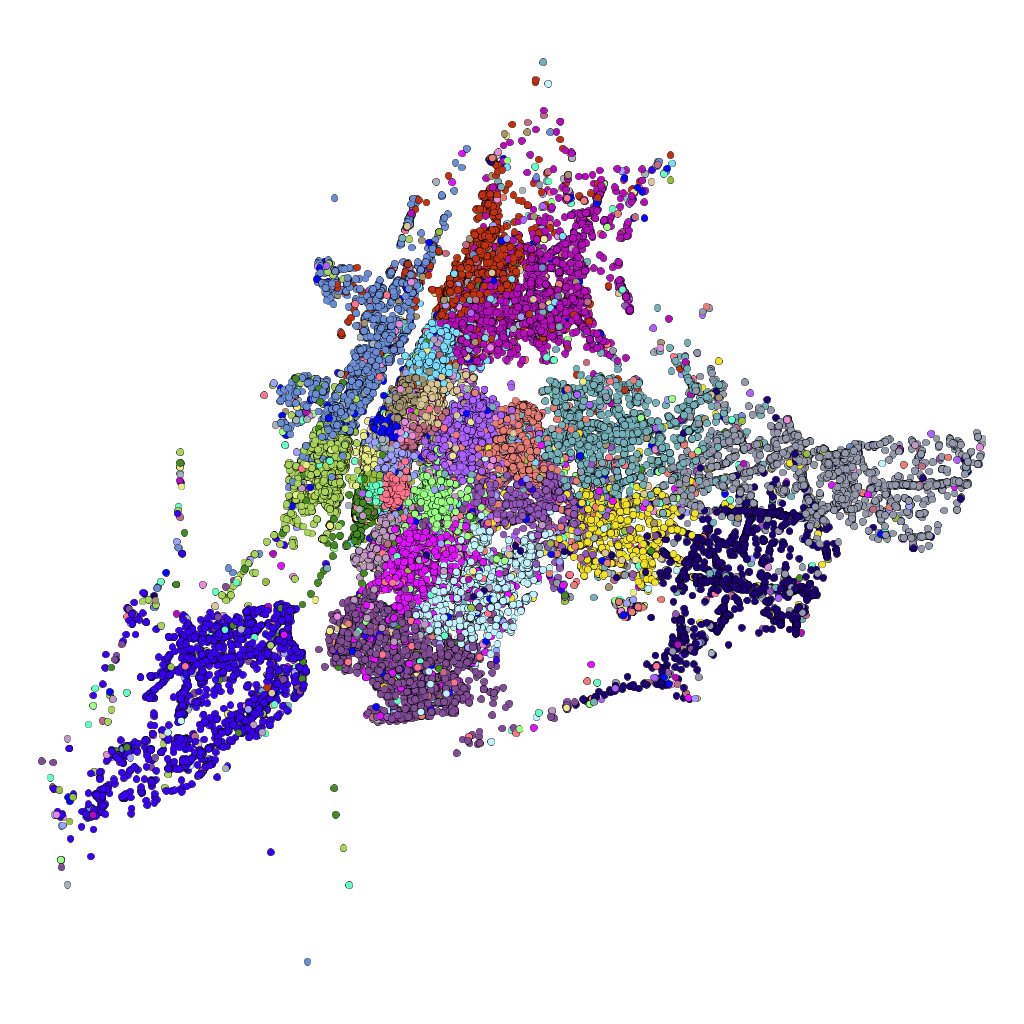
\includegraphics[width=\columnwidth]{../fsq_foo_2.png}
\caption{Foursquare venues coloured according to the community detected using the louvain method}
\label{fig:fsq-comm}
\end{figure}
\subsection{Foursquare neighbourhood for Airbnb Listing}
%I assign on each Airbnb listing the same Foursquare neighbourhood that the closest Foursquare venue to the listing belongs to. This is admittedly a very simple measure. Alternatively, one could consider multiple closest Foursquare venues and take the majority.
Let
\begin{align*}
S(l, n_{fsq}) = S(n_{fsq}) \cap k\_closest\_fsq(l, k)
\end{align*}
where $S(n_{fsq})$ returns a set of Foursquare venues which belong to a Foursquare neighbourhood $n_{fsq}$, and $k\_closest\_fsq(l, k)$ returns $k$ Foursquare venues which are closest to $l$. For a given Airbnb listing, I assign $n_{fsq}$ such that:
\begin{align*}
assign\_fsq\_nbh(l) = \argmax_{n_{fsq}} score(l, n_{fsq})
\end{align*}
where
\begin{align*}
score(l, n_{fsq}) =  \sum_{v \in S(l, n_{fsq})}distance(l, v)^{-1}
\end{align*}
Figure \ref{fig:abnb-comm} shows the Airbnb listings coloured according to the Foursquare neighbourhood they were assigned to, and Figure \ref{fig:abnb-nbh} shows the listings coloured according to the Airbnb neighbourhood they belong to. The colour used for each Foursquare neighbourhood is the same for both Figure \ref{fig:fsq-comm} and Figure \ref{fig:abnb-comm}. Note that Airbnb listings span over a much smaller region, which is why these figures look largely different from Figure \ref{fig:fsq-comm}. 
\begin{figure}
\centering
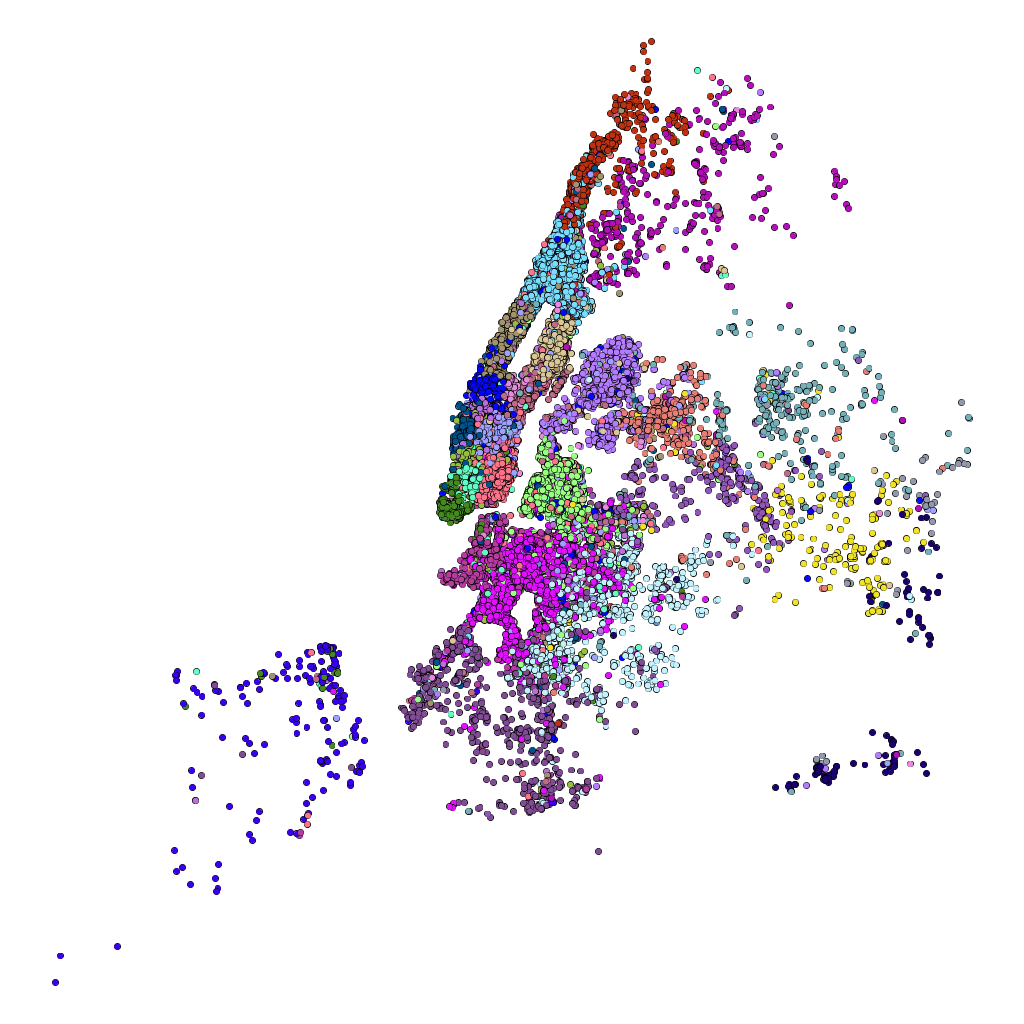
\includegraphics[width=\columnwidth]{../foo_3.png}
\caption{Airbnb listings coloured according to their Foursquare neighbourhood}
\label{fig:abnb-comm}
\end{figure}
\begin{figure}
\centering
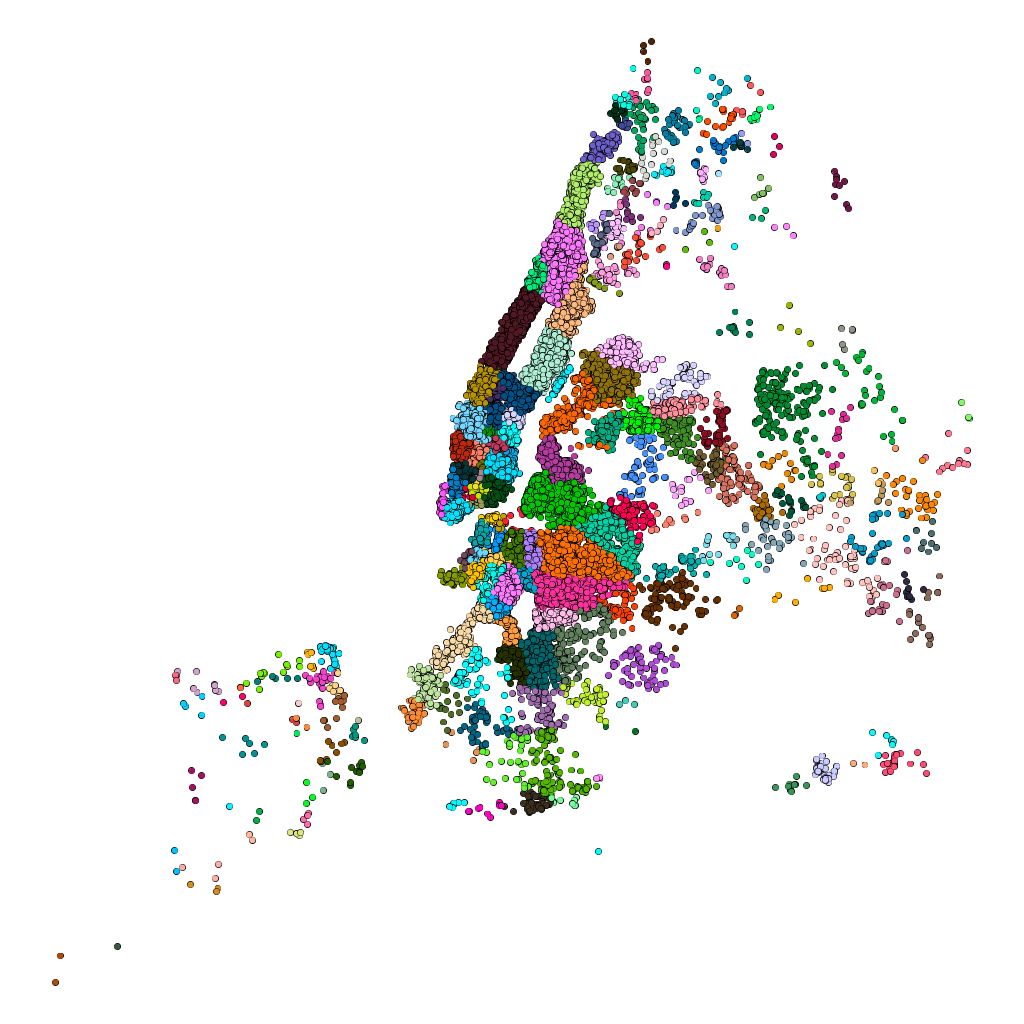
\includegraphics[width=\columnwidth]{../nbh_foo.png}
\caption{Airbnb listings coloured according to their Airbnb neighbourhood}
\label{fig:abnb-nbh}
\end{figure}
\subsection{Comparing Two Definitions}
First observation one can make is that the Airbnb neighbourhood is more fine-grained with 230 neighbourhoods than the Foursquare neighbourhood with 30 neighbourhoods. This is not due to the threshold value of 1000 venues that I used to filter the neighbourhoods. With the threshold of 1 venue, there would have been 180 neighbourhoods which are already fewer than the number of the Airbnb neighbourhoods. This may though be related to the rate of the decay of the weight with respect to the distance. For instance, if I chose to define $w_{i, j}$ to be inversely proportionate to $distance(i, j)^2$, the Foursquare neighbourhood potentially would have been more fine-grained.

Recall that there are more Foursquare neighbourhoods. One can say that these two definitions have a high overlap if a given Foursquare neighbourhood is such that it groups up multiple entire Airbnb neighbourhoods without splitting them. To quantify the overlap, I first assigned on each Airbnb neighbourhood a Foursquare neighbourhood to which the highest number of its listings were assigned to:
\begin{align*}
&assign\_fsq\_nbh(n_{a}) = \\
&\argmax_{n_fsq} | \{ l | l \in listings(n_{a}), assign\_fsq\_nbh(l) = n_{fsq}\} |
\end{align*}
where $listings(n_{a})$ returns a set of Airbnb listings which belong to $n_{a}$. Then I computed $overlap$ for the set of all the Airbnb listings $S_a$:
\begin{align*}
&overlap(S_a) = \\
& \frac{|\{ assign\_fsq\_nbh(l) = assign\_fsq\_nbh(nbh\_a(l)) | l \in S_a \}|}{|S_a|}
\end{align*}
where $nbh\_a(l)$ returns the Airbnb neighbourhood that $l$ belongs to.

As a result, I found that $overlap(S_a) = 0.653$, which is considerably higher than $3.33\mathrm{e}{-02}$ which what it would have been if a Foursquare neighbourhood was assigned at random on a listing. From this, we can conclude that Foursquare neighbourhood is such that it groups multiple Airbnb neighbourhoods and two definitions of neighbourhood somewhat overlaps.
\subsection{Popularity}
The total number of check-in is an indicator of the popularity of a Foursquare venue~\citep{noulas2011empirical}. One may consider an area to be a large Foursquare venue and naturally quantify its popularity as a sum of the number of check-in for Foursquare venues which belong to it. Let this measure of popularity of an area $n$ be $p_{fsq}(n)$.
On the contrary, there is no agreed way to quantify the popularity of an area using the information about Airbnb listings. In this section, I investigate various statistics of the Airbnb listings which belongs to an area, and see if any of them could be as good as $p_{fsq}(n)$ to quantify the popularity. I do this by computing the statistics on a Foursquare neighbourhood $n$ and measuring the correlation with $p_{fsq}(n)$.
\subsubsection{Candidate Statistics}
Intuitively, a listing is popular if there is more activity; that is, if it is occupied more frequently. Unfortunately, the Airbnb dataset does not offer such information. In the previous works, the activity of a listing was estimated by the number of reviews per month~\citep{cansoy2016gets, insideairbnb}. Airbnb guests may leave a review after their stay. Although it is optional and therefore not all the guests do so, this may be used as an indicator of Airbnb activity. 

Another possible indicator of the popularity of a listing would be the monthly income it generates. Again, this information is not available from the dataset. In the previous works, the minimum income per month was used instead. This can be computed as the product of the minimum length of stay, price and the reviews per month~\citep{cansoy2016gets, insideairbnb}. 

I propose the following statistics to measure the popularity of an area:
\begin{enumerate}
\item $p_{a1}(n)$\\ Average number of reviews per month given to the listings in an area $n$
\item $p_{a2}(n)$\\ Total number of reviews per month given to the listings in an area $n$
\item $p_{a3}(n)$\\ Average minimum income per month among the listings in an area $n$
\item $p_{a4}(n)$\\ Total minimum income per month earned by all the listings in an area $n$
\end{enumerate}
\label{sec:pop-measure}
\subsubsection{Results}
Figure \ref{fig:checkin_avg_reviews}, \ref{fig:checkin_ttl_reviews}, \ref{fig:checkin_avg_min_income} and \ref{fig:checkin_ttl_min_income} are scatter plots where each point represents a Foursquare neighbourhood. The x-coordinate represents its total check-in counts for the venues and the y-coordinate represents the respective candidate metric proposed in \ref{sec:pop-measure}.

There is no clear correlation between $p_{a1}(n)$ that can be read from Figure \ref{fig:checkin_avg_reviews}. The other statistics, though heteroskedastic, suggest a linear correlation with $p_{fsq}(n)$.

Table \ref{tab:pop-corr} shows Pearson's correlation coefficient $r$ and p-value $p$ between each candidate proposed in \ref{sec:pop-measure} and $p_{fsq}$.
Taking the threshold value of 0.01, only $p_{a3}$ and $p_{a4}$ are significantly correlated to $p_{fsq}$. From this we can conclude that a good statistic which can be obtained from the Airbnb dataset to measure the popularity of an area is either $p_{a3}$ or $p_{a4}$, though the lower p-value for $p_{a3}$ suggests that $p_{a3}$ is a better statistic for this purpose, assuming that $p_{fsq}$ is indeed a good measure of the popularity of an area.

There are two possible reason why $p_{a3}$ and $p_{a4}$ are better suited for measuring the popularity of an area than $p_{a1}$ and $p_{a2}$. One is that the number of reviews per month of a listing may be influenced much more than the popularity of the area, such as the demographics or the purpose of the visits of the guests.

Though the minimum income per month is not independent of these factors, as it is after all defined in terms of the number of reviews per month, the noise introduced might be offset by other variables introduced, which are the price and the minimum length of stay, which possibly has a high correlation with $p_{fsq}$.

% THIS LED ME TRY ..
Figure \ref{fig:checkin_avg_price} and \ref{fig:checkin_avg_length} are scatter plots where each point represents a Foursquare neighbourhood. The x-axis is again the total check-in counts of the venues in the neighbourhood and the y-axis is the average price of the and the average minimum length of stay of a listing, respectively. Unsurprisingly, the average minimum length of stay seems to be invariant of $p_{fsq}$. The average price though seems to have a linear correlation with $p_{fsq}$.  Indeed Pearson's correlation coefficient between the average price and $p_{fsq}$ is $0.742$ with p-value of $ 2.68\mathrm{e}{-06}$, which is lower than that of $p_{a4}$. 
From this we can conclude that the average price of the listing is the best indicator of the popularity of the area. This result goes well with the intuition that a guest would be willing to pay more to be in a popular area.

\begin{figure}
\centering
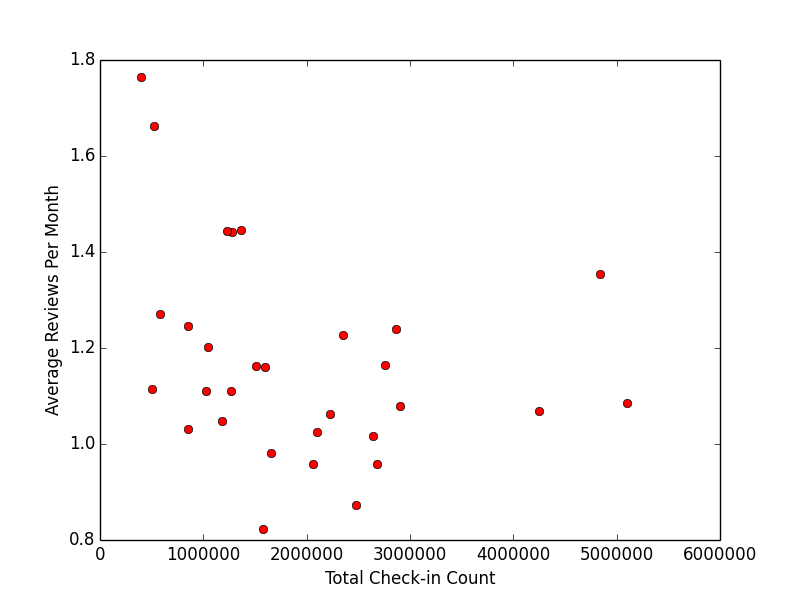
\includegraphics[width=\columnwidth]{../checkin_avg_reviews.png}
\caption{Total Check-in Count and Average Reviews Per Month of Foursquare Neighbourhoods ($p_{a1}(n)$ against $p_{fsq}(n)$)}
\label{fig:checkin_avg_reviews}
\end{figure}
\begin{figure}
\centering
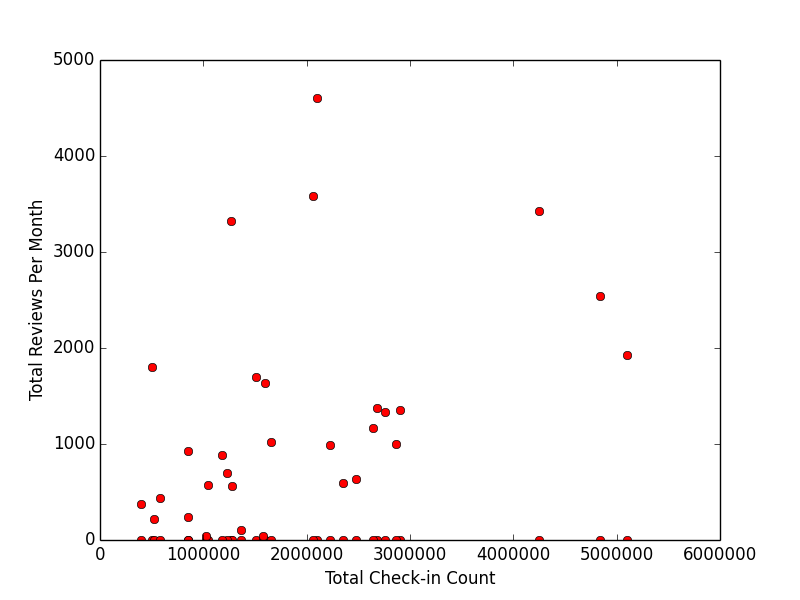
\includegraphics[width=\columnwidth]{../checkin_ttl_reviews.png}
\caption{Total Check-in Count and Total Reviews Per Month of Foursquare Neighbourhoods ($p_{a2}(n)$ against $p_{fsq}(n)$)}
\label{fig:checkin_ttl_reviews}
\end{figure}
\begin{figure}
\centering
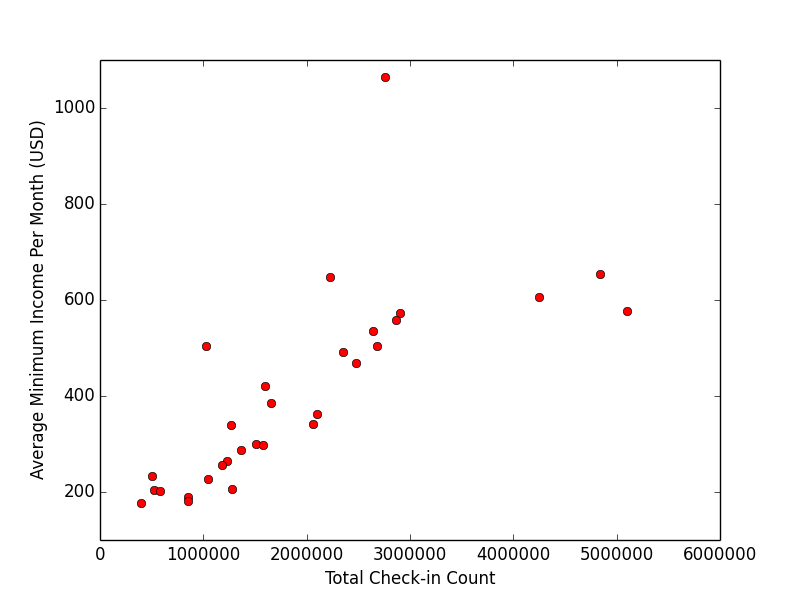
\includegraphics[width=\columnwidth]{../checkin_avg_min_income.png}
\caption{Total Check-in Count and Average Minimum Income Per Month of Foursquare Neighbourhoods ($p_{a3}(n)$ against $p_{fsq}(n)$))} 
\label{fig:checkin_avg_min_income}
\end{figure}
\begin{figure}
\centering
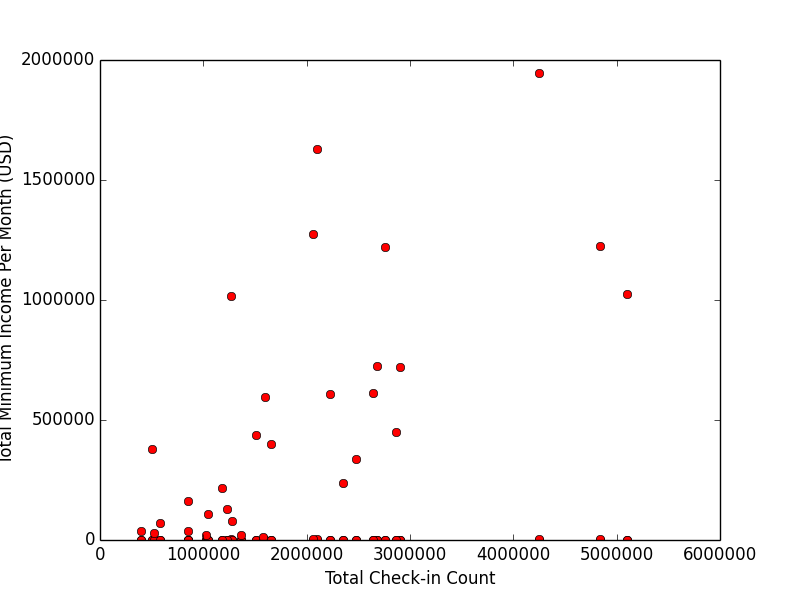
\includegraphics[width=\columnwidth]{../checkin_ttl_min_income.png}
\caption{Total Check-in Count and Total Minimum Income Per Month of Foursquare Neighbourhoods ($p_{a4}(n)$ against $p_{fsq}(n)$)}
\label{fig:checkin_ttl_min_income}
\end{figure}
\begin{table}[]
\centering
\caption{Pearson's Correlation Coefficient $r$ and p-value $p$}
\label{tab:pop-corr}
\begin{tabular}{|l|l|l|}
\hline
         & $r$ & $p$ \\ \hline
$p_{a2}$ &  0.439 & $1.53\mathrm{e}{-02}$     \\ \hline
$p_{a3}$ &  0.728   & $5.07\mathrm{e}{-06}$  \\ \hline
$p_{a4}$ & 0.697 & $1.88\mathrm{e}{-05}$     \\ \hline
\end{tabular}
\end{table}
\begin{figure}
\centering
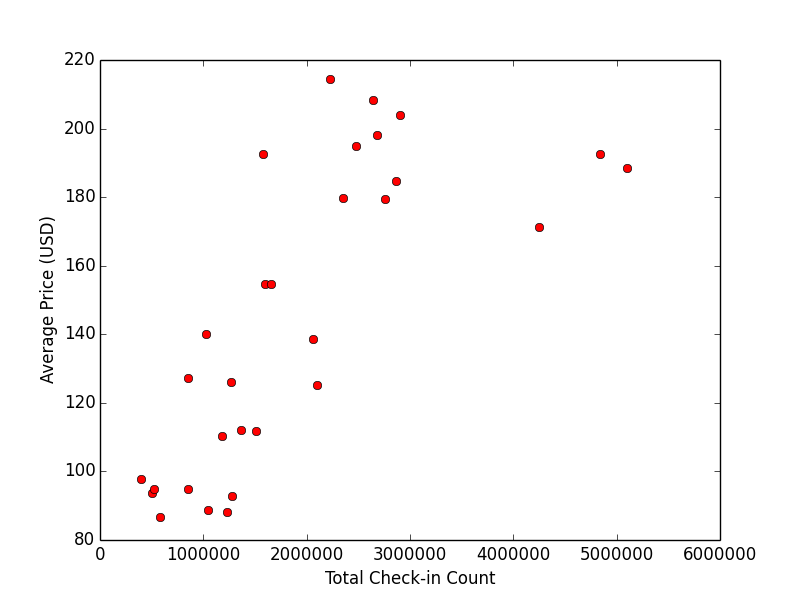
\includegraphics[width=\columnwidth]{../checkin_avg_price.png}
\caption{Total Check-in Count and Average Price of Listings in Foursquare Neighbourhoods}
\label{fig:checkin_avg_price}
\end{figure}
\begin{figure}
\centering
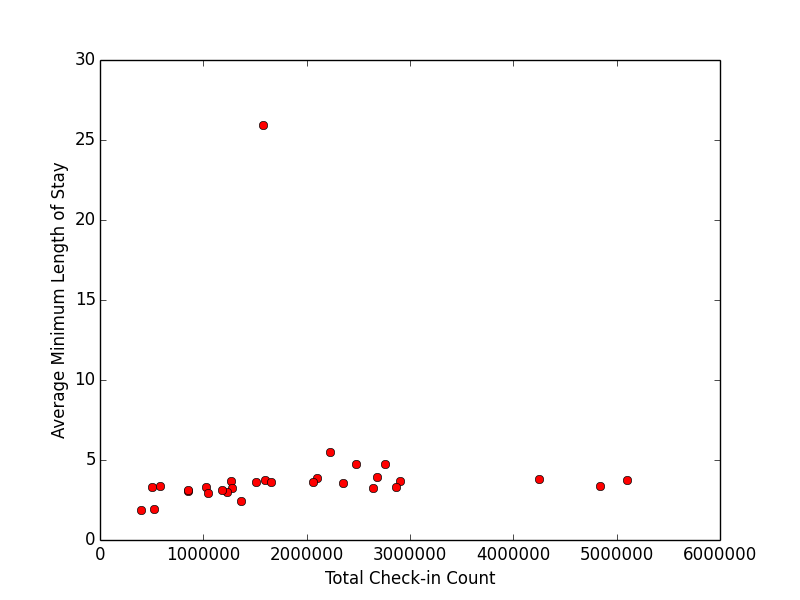
\includegraphics[width=\columnwidth]{../checkin_avg_length.png}
\caption{Total Check-in Count and Average Minimum of Length of Stay of Listings in Foursquare Neighbourhoods}
\label{fig:checkin_avg_length}
\end{figure}